\documentclass[12pt,a4paper]{article}

\usepackage[T1]{fontenc}
\usepackage[utf8]{inputenc}
\usepackage[margin=2.5cm]{geometry}
\usepackage{lmodern}
\usepackage{microtype}
\usepackage{parskip}
\usepackage{titlesec}
\usepackage{booktabs}
\usepackage{xcolor}
\usepackage{hyperref}
\usepackage{listings}
\usepackage{tikz}
\usetikzlibrary{shapes,arrows,positioning,fit,backgrounds,calc}

\definecolor{mpblue}{HTML}{1A73E8}
\definecolor{mpgreen}{HTML}{34A853}
\definecolor{mporange}{HTML}{EA8600}
\definecolor{mppurple}{HTML}{9C27B0}
\definecolor{mpgray}{HTML}{5F6368}
\definecolor{mpred}{HTML}{EA4335}
\definecolor{codebg}{HTML}{F8F9FA}
\definecolor{codeframe}{HTML}{DADCE0}

\hypersetup{colorlinks=true, linkcolor=mpblue, urlcolor=mpblue,
    pdftitle={MediaPipe Tutorial 05 -- Object Detection}}

\lstdefinestyle{pythonstyle}{
    language=Python, backgroundcolor=\color{codebg},
    frame=single, framerule=0.8pt, rulecolor=\color{codeframe},
    basicstyle=\ttfamily\small,
    keywordstyle=\color{mpblue}\bfseries,
    stringstyle=\color{mpgreen},
    commentstyle=\color{mpgray}\itshape,
    numberstyle=\tiny\color{mpgray},
    numbers=left, numbersep=8pt,
    breaklines=true, showstringspaces=false, tabsize=4,
}
\lstset{style=pythonstyle}

\titleformat{\section}{\large\bfseries\color{mpblue}}{}{0em}{}[\titlerule]
\titleformat{\subsection}{\normalsize\bfseries\color{mpgray}}{}{0em}{}

\tikzset{
    arch/.style={rectangle, rounded corners=4pt,
        draw=#1, fill=#1!12,
        text width=2.6cm, align=center,
        minimum height=1.2cm, font=\small\bfseries},
    archarrow/.style={->, >=stealth, thick, color=#1},
    archlabel/.style={font=\footnotesize, color=mpgray, align=center},
}

\begin{document}

\title{\textbf{\textcolor{mpblue}{MediaPipe Tutorial 05}}\\[0.4em]
    \large Object Detection: EfficientDet-Lite, Bounding Boxes,\\
    NMS Tuning, Centroid Tracking, and FPS Benchmarks}
\author{MediaPipe Tutorials Series}
\date{\today}
\maketitle
\tableofcontents
\newpage

% ─────────────────────────────────────────────────────────────────────────────
\section{Introduction}

EfficientDet-Lite detects and classifies objects from 90 COCO categories in real time.
This tutorial covers model selection, bounding-box drawing, NMS tuning, a centroid tracker
for stable IDs, and FPS benchmarks across hardware.

% ─────────────────────────────────────────────────────────────────────────────
\section{EfficientDet Architecture Diagram}

\bigskip

\begin{center}
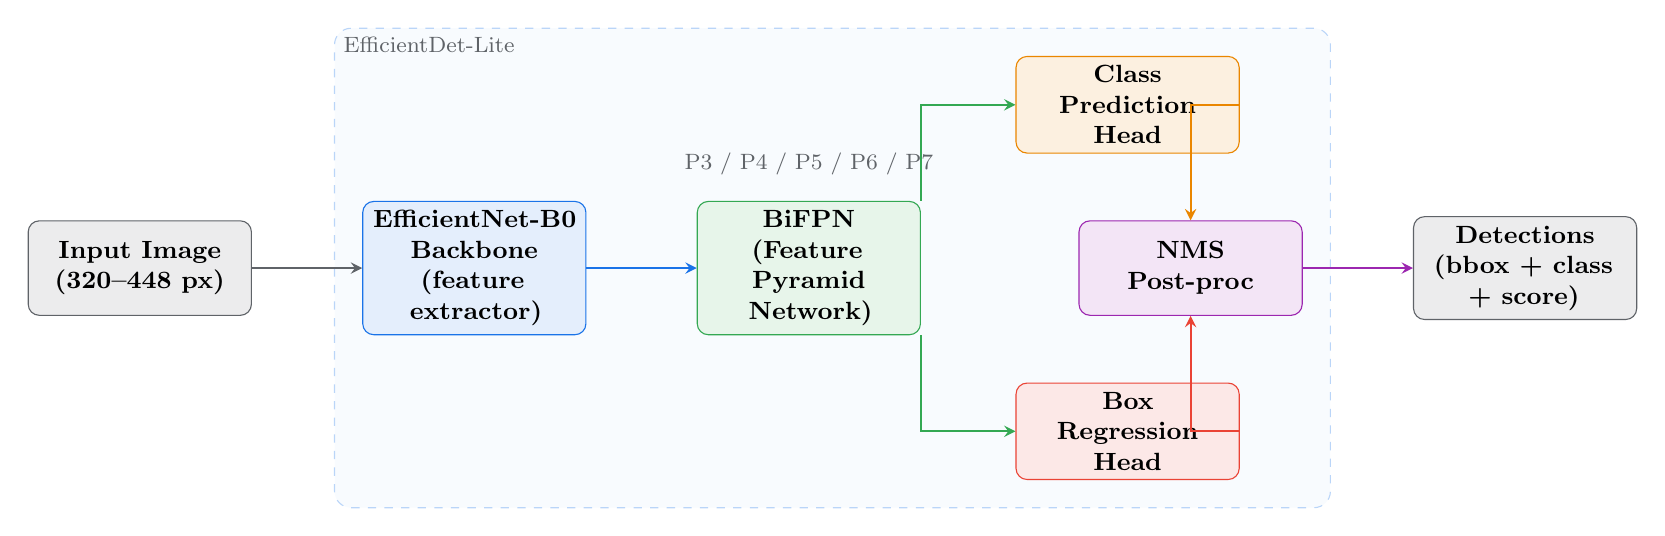
\begin{tikzpicture}[node distance=1.0cm and 1.4cm]

    % ── Input ──────────────────────────────────────────────────────────────
    \node[arch=mpgray] (input)
        {Input Image\\(320--448 px)};

    % ── Backbone ───────────────────────────────────────────────────────────
    \node[arch=mpblue, right=of input] (backbone)
        {EfficientNet-B0\\Backbone\\(feature extractor)};

    % ── Multi-scale feature maps ────────────────────────────────────────────
    \node[arch=mpgreen, right=of backbone] (fpn)
        {BiFPN\\(Feature Pyramid\\Network)};

    % ── Class / box heads ──────────────────────────────────────────────────
    \node[arch=mporange, above right=0.6cm and 1.2cm of fpn] (cls_head)
        {Class\\Prediction\\Head};
    \node[arch=mpred, below right=0.6cm and 1.2cm of fpn] (box_head)
        {Box\\Regression\\Head};

    % ── NMS ────────────────────────────────────────────────────────────────
    \node[arch=mppurple, right=2.0cm of fpn] (nms)
        {NMS\\Post-proc};

    % ── Output ─────────────────────────────────────────────────────────────
    \node[arch=mpgray, right=of nms] (output)
        {Detections\\(bbox + class\\+ score)};

    % ── Arrows ─────────────────────────────────────────────────────────────
    \draw[archarrow=mpgray]   (input)    -- (backbone);
    \draw[archarrow=mpblue]   (backbone) -- (fpn);
    \draw[archarrow=mpgreen]  (fpn.north east) |- (cls_head.west);
    \draw[archarrow=mpgreen]  (fpn.south east) |- (box_head.west);
    \draw[archarrow=mporange] (cls_head.east) -| (nms.north);
    \draw[archarrow=mpred]    (box_head.east) -| (nms.south);
    \draw[archarrow=mppurple] (nms) -- (output);

    % ── FPN scale labels ────────────────────────────────────────────────────
    \node[archlabel, above=0.2cm of fpn] {P3 / P4 / P5 / P6 / P7};

    % ── Background frame ────────────────────────────────────────────────────
    \begin{scope}[on background layer]
        \node[draw=mpblue!30, dashed, rounded corners=6pt,
              fill=mpblue!3,
              fit=(backbone)(fpn)(cls_head)(box_head)(nms),
              inner sep=10pt,
              label={[archlabel, anchor=north west]north west:EfficientDet-Lite}
              ] {};
    \end{scope}

\end{tikzpicture}
\end{center}

\bigskip

% ─────────────────────────────────────────────────────────────────────────────
\section{Model Comparison}

\begin{center}
\begin{tabular}{llccc}
\toprule
\textbf{Model} & \textbf{File} & \textbf{mAP} & \textbf{Latency (Pixel 6)} & \textbf{Input size} \\
\midrule
Lite0 & \texttt{efficientdet\_lite0.tflite} & 25.6\% & 37 ms  & 320$\times$320 \\
Lite1 & \texttt{efficientdet\_lite1.tflite} & 30.5\% & 49 ms  & 384$\times$384 \\
Lite2 & \texttt{efficientdet\_lite2.tflite} & 33.5\% & 69 ms  & 448$\times$448 \\
\bottomrule
\end{tabular}
\end{center}

% ─────────────────────────────────────────────────────────────────────────────
\section{Real-Time Object Detection}

\begin{lstlisting}[caption={Tasks API object detector}]
import cv2, mediapipe as mp, time
from mediapipe.tasks import python as mp_python
from mediapipe.tasks.python import vision

model_path = "efficientdet_lite0.tflite"
base_opts = mp_python.BaseOptions(model_asset_path=model_path)
options = vision.ObjectDetectorOptions(
    base_options=base_opts,
    running_mode=vision.RunningMode.VIDEO,
    score_threshold=0.45,
    max_results=10,
)
cap = cv2.VideoCapture(0)
with vision.ObjectDetector.create_from_options(options) as detector:
    ts = 0
    while cap.isOpened():
        ret, frame = cap.read()
        if not ret: break
        ts += 33
        mp_img = mp.Image(image_format=mp.ImageFormat.SRGB,
                          data=cv2.cvtColor(frame, cv2.COLOR_BGR2RGB))
        result = detector.detect_for_video(mp_img, ts)
        for det in result.detections:
            bb = det.bounding_box
            cv2.rectangle(frame,
                (bb.origin_x, bb.origin_y),
                (bb.origin_x+bb.width, bb.origin_y+bb.height),
                (0,255,0), 2)
        cv2.imshow("Detect", frame)
        if cv2.waitKey(1) & 0xFF == ord('q'): break
cap.release(); cv2.destroyAllWindows()
\end{lstlisting}

% ─────────────────────────────────────────────────────────────────────────────
\section{FPS Benchmark}

\begin{center}
\begin{tabular}{llc}
\toprule
\textbf{Platform} & \textbf{Accelerator} & \textbf{FPS (Lite0)} \\
\midrule
Intel i9-12900K   & CPU (4 threads)   & 38 \\
NVIDIA RTX 3060   & CUDA              & 85 \\
Google Coral      & Edge TPU          & 110 \\
Apple M2 Pro      & CPU               & 55 \\
Apple M2 Pro      & Metal (GPU)       & 95 \\
Raspberry Pi 4B   & ARM Cortex-A72    & 8  \\
\bottomrule
\end{tabular}
\end{center}

% ─────────────────────────────────────────────────────────────────────────────
\section{Next Steps}

Proceed to Tutorial~06 to apply image segmentation for background replacement
and virtual green-screen effects.

\end{document}
